\section{Giai đoạn 1: Thu thập dữ liệu đa nguồn và tối ưu lưu trữ}

\subsection{Chiến lược dò tìm bài báo và thu hoạch lịch sử phiên bản}

Bài toán xác định trọn vẹn tập bài báo hợp lệ trong mỗi dải mã arXiv được giao không đơn thuần là phép tăng số tuần tự, đặc biệt khi dải mã bắc ngang ranh giới hai tháng dương lịch. Theo quy ước định danh của arXiv, bộ đếm năm chữ số sẽ đặt lại về $00001$ vào ngày đầu mỗi tháng trong khi ngưỡng số thứ tự cuối cùng của tháng trước đó không cố định và không có giao diện tra cứu trực tiếp~\cite{arxiv_api}. Thay vì ước đoán ngưỡng kết thúc tháng hoặc dừng sớm khi gặp một vài khe mã bị rút bài, phân hệ dò tìm tạo danh sách ứng viên theo từng lô $100$ mã và quét cạn tới $99{,}999$ của tháng mở đầu trước khi chuyển sang $00001$ của tháng kế tiếp. Chính cơ chế quét an toàn này giải thích vì sao hai dải xuyên tháng phải kiểm định $83{,}142$ mã (từ $2504.17523$ đến $2504.99999$ cộng $665$ mã tháng $05/2025$) và $80{,}870$ mã (từ $2506.20788$ đến $2506.99999$ cộng $1{,}658$ mã tháng $07/2025$) thay vì đúng $5{,}000$ mã như ba dải nội tháng. Mọi truy vấn gửi tới cổng tìm kiếm Atom của arXiv đều tuân thủ nghiêm ngặt quy tắc một kết nối đơn với khoảng nghỉ tối thiểu $3\text{ giây}$ giữa hai lần gọi~\cite{arxiv_api}. Nhằm ngăn ngừa kết luận sai rằng bài báo không tồn tại khi máy chủ trả phản hồi cắt xén, bộ phân tích chỉ chấp nhận suy diễn vắng mặt khi thỏa đồng thời bất biến đầy đủ phân trang: chỉ số khởi đầu phản hồi bằng $0$ và tổng số kết quả khai báo trùng khớp tuyệt đối với số mục thực nhận trong tài liệu XML. Bất cứ lô truy vấn nào xuất hiện sai lệch số lượng, thiếu thẻ phân trang hoặc cấu trúc bất thường đều tự động chuyển sang chế độ truy vấn đơn lẻ cho từng mã ứng viên, đồng thời áp đặt giới hạn kích thước gói phản hồi và vô hiệu hóa cơ chế mở rộng thực thể XML ngoài nhằm phòng ngừa tấn công tiêm thực thể và tràn bộ nhớ.

Mặc dù giao diện Atom đáp ứng tốt bài toán phát hiện sự tồn tại của bài báo, dịch vụ này chỉ công bố hai mốc thời gian là ngày nộp đầu tiên và ngày cập nhật gần nhất, làm thất lạc hoàn toàn lịch sử các phiên bản trung gian $v_2, \dots, v_{N-1}$. Trong kho dữ liệu thực tế của nhóm, có tới $42.64\%$ bài báo sở hữu từ hai phiên bản trở lên (tối đa tới $v_{13}$), khiến việc dùng Atom cho thu hoạch siêu dữ liệu trở nên bất khả thi đối với yêu cầu bảo toàn nguồn gốc thời gian ở mức phiên bản. Do đó, hệ thống chuyển công đoạn thu hoạch siêu dữ liệu sang giao thức OAI-PMH trên điểm cuối đám mây mới mà arXiv chính thức di chuyển từ tháng $03/2025$~\cite{arxiv_oai_2025}, sử dụng định dạng siêu dữ liệu gốc đầy đủ của arXiv để lấy đồng thời danh sách trọn vẹn từng phiên bản kèm dấu thời gian chính xác và thông tin nơi công bố chính thức. Do chuỗi danh sách tác giả thô trên arXiv thường trộn lẫn tên đơn vị công tác trong dấu ngoặc đơn, cụm dấu ngoặc nhọn chứa dấu phụ LaTeX, hậu tố thế hệ sau dấu phẩy và tên tổ hợp nghiên cứu, bộ chuẩn hóa tác giả tất định thực hiện tách theo nhiều bước: loại bỏ chú thích đơn vị trong ngoặc đơn, bảo toàn khối ngoặc nhọn cân bằng khi tách dấu phẩy, gắn lại hậu tố thế hệ vào họ tác giả liền trước và tách riêng tiền tố nhóm hợp tác. Toàn bộ mốc thời gian thu nhận từ cả OAI-PMH lẫn Atom đều được quy đổi về định dạng chuẩn giờ phối hợp quốc tế UTC có gắn thông tin múi giờ nhằm loại trừ sai lệch đồng hồ cục bộ khi đối chiếu chuỗi phiên bản và ngày trích dẫn về sau.

\subsection{Tải mã nguồn toàn văn đa định dạng và lọc bỏ tài nguyên nhị phân}

Công đoạn tải toàn văn mã nguồn cho từng phiên bản bài báo được định tuyến tuyệt đối về máy chủ gương xuất dữ liệu chuyên dụng của arXiv thay vì truy cập cổng web công cộng, kèm theo tiêu đề định danh tác nhân khách mô tả rõ danh tính học thuật và chu kỳ giãn cách $3\text{ giây}$ nhằm tôn trọng chính sách tải hàng loạt~\cite{arxiv_api}. Mỗi phiên tải áp đặt kiểm tra mã trạng thái HTTP $200$ trọn vẹn, từ chối rõ ràng các phản hồi phân đoạn HTTP $206$ vốn có thể âm thầm cắt cụt dòng nén, đồng thời duy trì ngưỡng giới hạn dung lượng đọc luồng để tránh làm kiệt quệ bộ nhớ máy ảo trước các gói nén dị thường. Do điểm cuối xuất mã nguồn của arXiv phục vụ nhiều định dạng nộp bài khác nhau dưới cùng một cấu trúc đường dẫn mà không bảo đảm độ tin cậy của tiêu đề kiểu nội dung, tầng tiếp nhận không dựa vào đuôi tên tệp mà thực hiện nhận diện chữ ký byte mở đầu kết hợp kiểm tra tiêu đề cấu trúc tệp. Cơ chế nhận diện đa tầng này phân loại chính xác mọi gói tải về vào sáu nhóm định dạng thực tế: gói nén tar dùng thuật toán gzip, gói tar không nén, tệp văn bản TeX nén đơn bằng gzip, tệp văn bản TeX thuần không nén, bài nộp chỉ gồm tài liệu PDF và tài liệu soạn thảo theo chuẩn Office Open XML. Nhờ tách biệt việc nhận diện nhị phân khỏi phần mở rộng đường dẫn, bộ tiếp nhận xử lý an toàn cả các luồng nén lồng nhau lẫn tệp văn bản thuần bị gắn nhãn nén sai lệch. Quy trình phối hợp giữa dò tìm, thu hoạch siêu dữ liệu, nhận diện định dạng, lọc nguồn và xuất bản nguyên tử được tổng hợp trực quan trong Hình~\ref{fig:m1_crawling_flow}.

\begin{figure}[htbp]
    \centering
    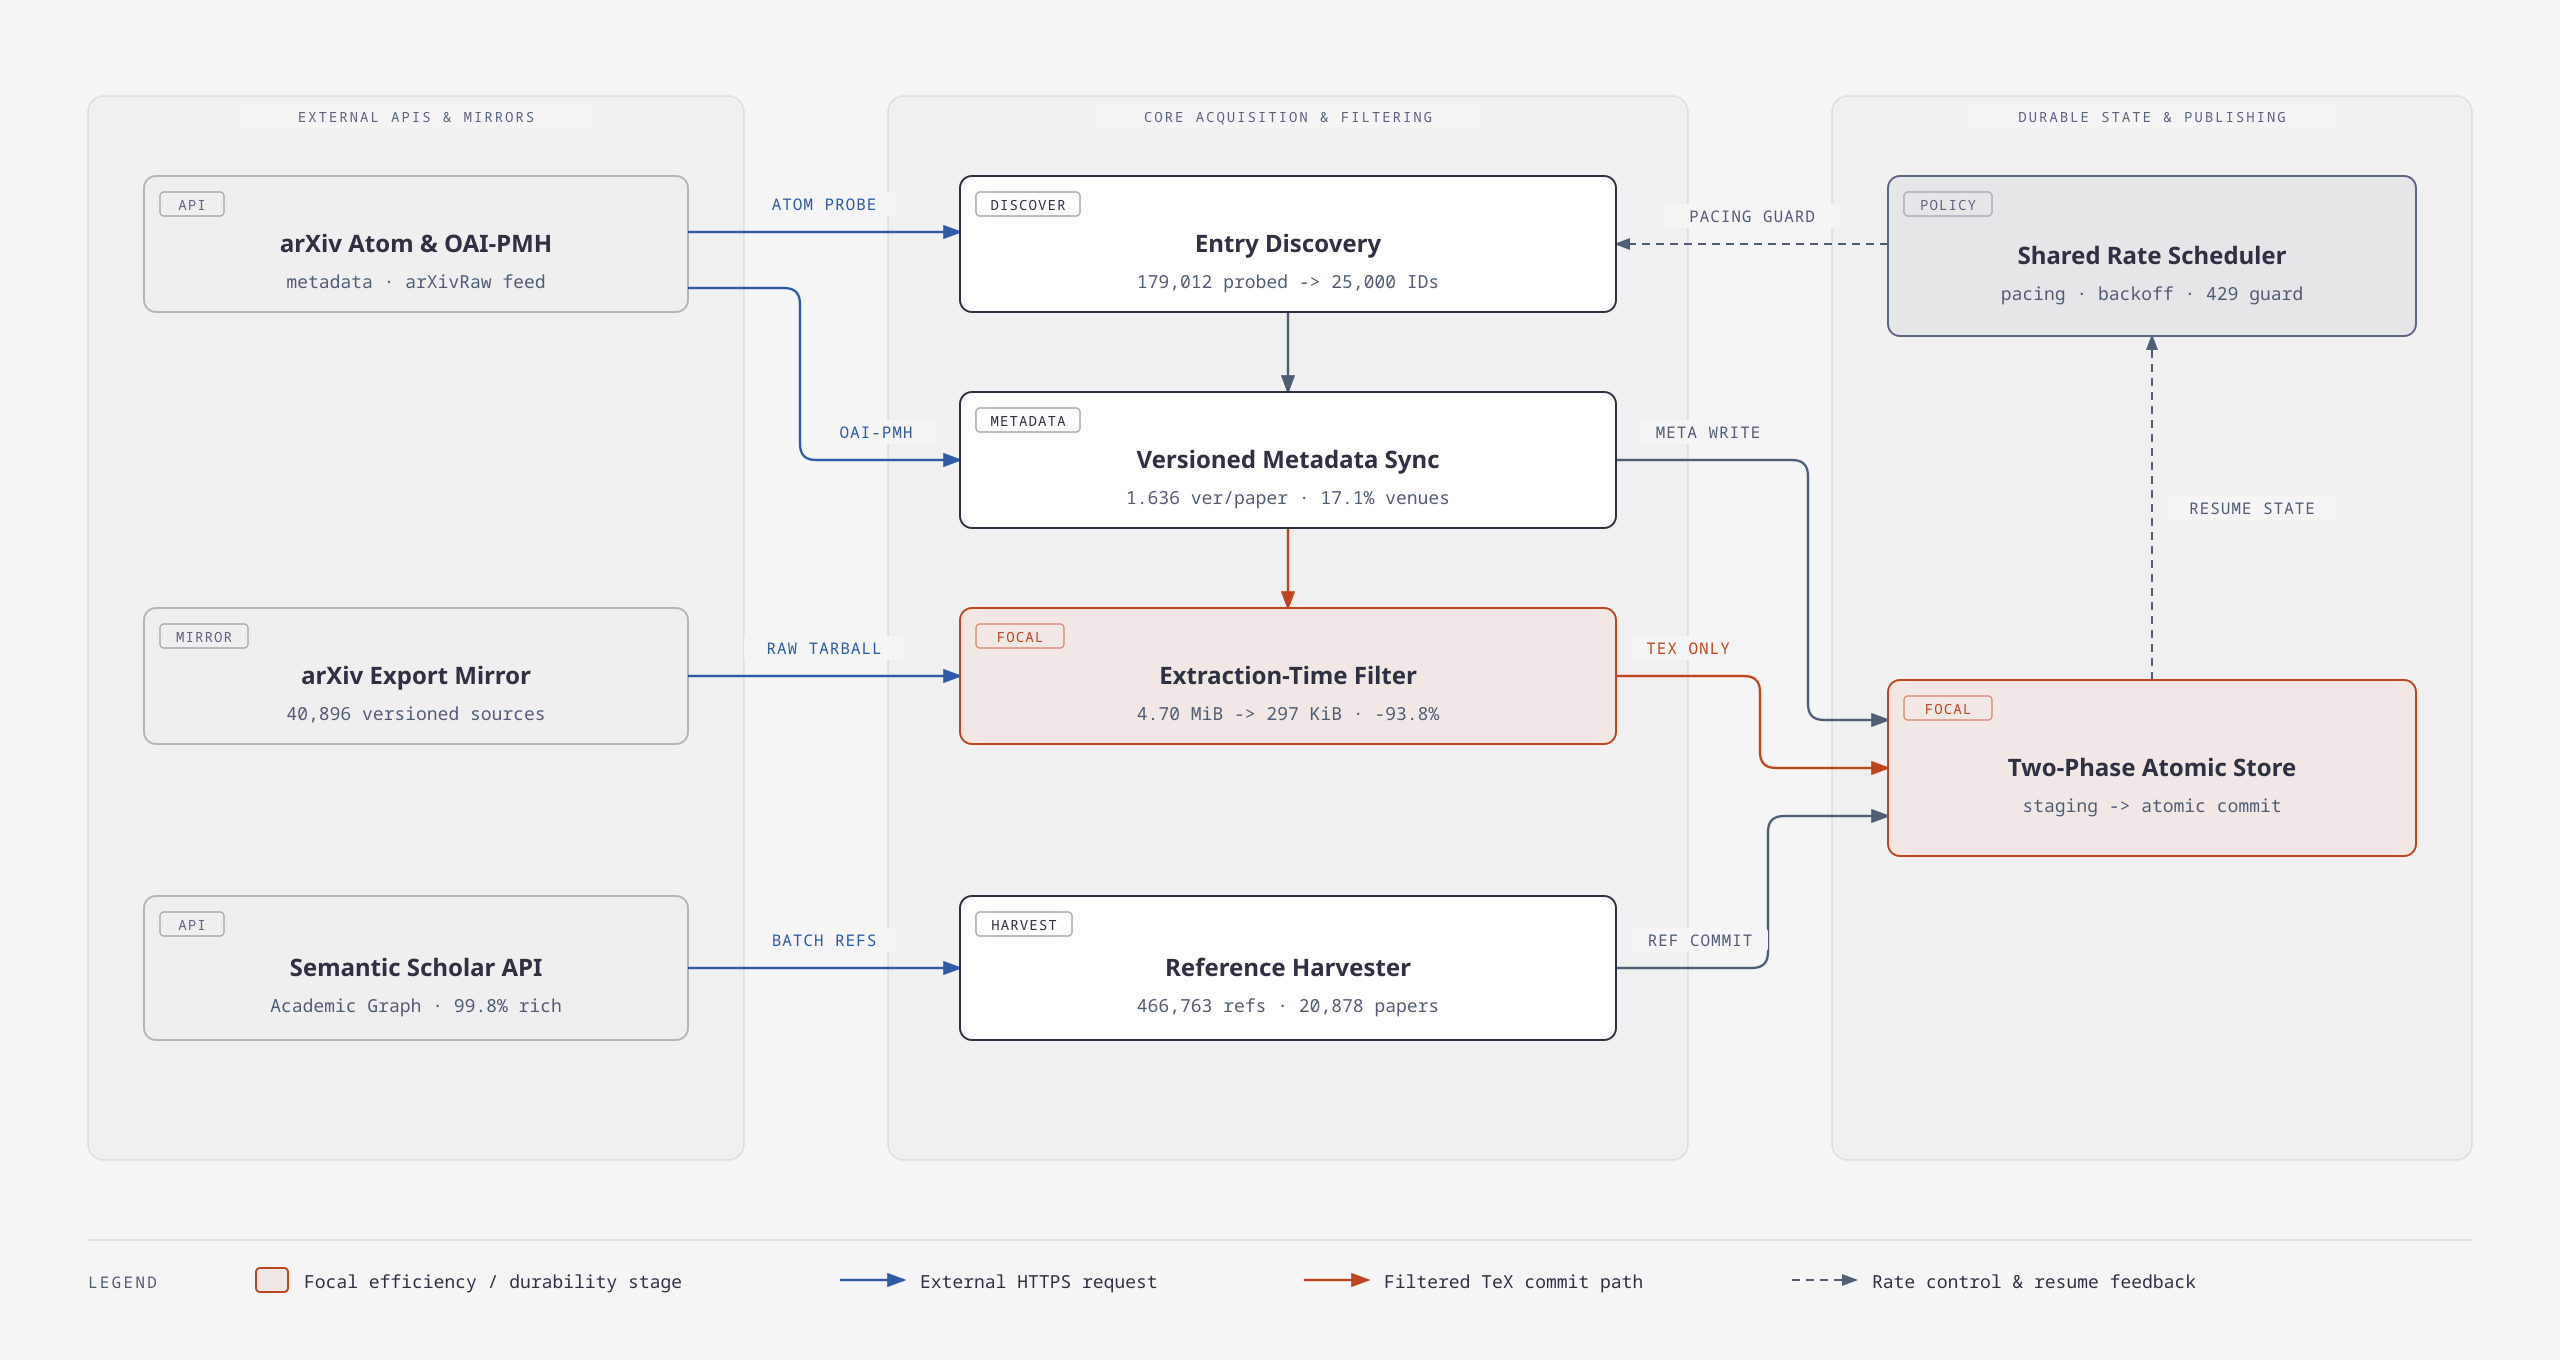
\includegraphics[width=\linewidth]{images/m1_crawling_flow.png}
    \caption[Quy trình thu thập dữ liệu đa nguồn và tối ưu lưu trữ ở Giai đoạn 1]{Quy trình thu thập dữ liệu đa nguồn và tối ưu lưu trữ ở Giai đoạn 1: dò tìm lô xuyên ranh giới tháng, thu hoạch lịch sử phiên bản OAI-PMH, nhận diện sáu định dạng và lọc chọn lọc ngay lúc giải nén, thu hoạch mạng trích dẫn Semantic Scholar có khắc phục lỗi tiêu đề khóa API và xuất bản giao dịch hai pha.}
    \label{fig:m1_crawling_flow}
\end{figure}

Phần lớn dung lượng của một gói mã nguồn bài báo khoa học trên arXiv đến từ hình ảnh độ phân giải cao, đồ thị vectơ và các tệp dữ liệu nhị phân phụ trợ. Nếu lưu nguyên trạng toàn bộ $40{,}896$ phiên bản, kho lưu trữ sẽ tiêu tốn xấp xỉ $200\text{ GiB}$ và nhanh chóng vượt quá dung lượng của môi trường đám mây phổ thông. Để giải quyết triệt để nút thắt lưu trữ mà không ảnh hưởng đến tính nguyên vẹn văn bản, bộ lọc hoạt động trực tiếp tại thời điểm giải nén và chỉ giữ lại nguyên vẹn từng byte các tệp mã nguồn TeX cùng tệp thư mục BibTeX, tuyệt đối không chỉnh sửa hay xóa bỏ các lệnh chèn hình ảnh hoặc bảng biểu bên trong mã TeX để bảo toàn nguyên trạng ngữ cảnh phân tích cho Giai đoạn 2. Trước khi giải nén bất kỳ thành phần nào trong gói lưu trữ, hàng rào bảo mật sẽ từ chối liên kết mềm, liên kết cứng, đường dẫn tuyệt đối và chuỗi vượt cấp thư mục cha, kiểm định mã kiểm tra vòng CRC ở phần đuôi dòng gzip chống lỗi hỏng dữ liệu, đồng thời giới hạn số lượng tệp cùng tổng kích thước bung nén nhằm vô hiệu hóa nguy cơ bom giải nén. Với mọi phiên bản có mã nguồn hợp lệ, quá trình lọc phải thỏa mãn bất biến hạch toán dung lượng chính xác tại Phương trình~\eqref{eq:m1_byte_accounting} giữa tổng kích thước gói tải về $B_{\text{raw}}$, dung lượng mã nguồn giữ lại $B_{\text{src}}$, dung lượng tài nguyên nhị phân loại bỏ $B_{\text{bin}}$ và phần phụ trội cấu trúc gói nén $B_{\text{ovh}}$:
\begin{equation}
    B_{\text{raw}} = B_{\text{src}} + B_{\text{bin}} + B_{\text{ovh}}, \qquad
    \rho_{\text{save}} = 1 - \frac{B_{\text{src}}}{B_{\text{raw}}}.
    \label{eq:m1_byte_accounting}
\end{equation}
Đối với khoảng $5.38\%$ đến $7.28\%$ phiên bản không chứa mã nguồn TeX (chủ yếu là bài nộp PDF thuần hoặc tài liệu Office Open XML, nhất quán với mức bao phủ nguồn TeX khoảng $97\%$ cùng tỷ lệ ngoại lệ trên toàn kho arXiv~\cite{ginev2024}), hệ thống kiên quyết không xóa bỏ bài báo mà vẫn ghi nhận hồ sơ nguồn rỗng có đánh dấu trạng thái rõ ràng nhằm giữ vẹn toàn tập hợp $25{,}000$ bài báo chính thức xuyên suốt mọi bảng thống kê.

\subsection{Khai thác mạng lưới trích dẫn, khắc phục giới hạn tần suất và cơ chế bền vững}

Để tạo tập ứng viên tài liệu tham khảo đầu vào cho bài toán đối sánh có giám sát ở Giai đoạn 3, phân hệ thu thập trích dẫn tích hợp với giao diện lập trình đồ thị học thuật của Semantic Scholar~\cite{kinney2023}, nền tảng đạt độ chính xác trích xuất tài liệu tham khảo trên $90\%$ trong xây dựng đồ thị văn học khoa học~\cite{ammar2018}. Các truy vấn chỉ yêu cầu tập trường thư mục dạng phẳng nhằm thu gọn băng thông truyền tải trong khi vẫn lưu trữ đầy đủ toàn bộ danh sách trích dẫn thô tại kho cục bộ để phục vụ đối chiếu kiểm toán khi cần thiết. Khi xuất bản dữ liệu cho giai đoạn đối sánh, hệ thống lọc lấy các tài liệu tham khảo sở hữu mã định danh ngoài của arXiv, bảo toàn cẩn trọng cả định dạng số mới lẫn định dạng tiền năm $2007$ có tiền tố lĩnh vực kèm dấu gạch chéo ($\text{lĩnh vực}/\text{YYMMNNN}$). Một sai lệch ngữ nghĩa nghiêm trọng thường gặp ở bước này là trường ngày công bố trên Semantic Scholar thường phản ánh ngày xuất bản tại tạp chí hoặc hội nghị (có thể trễ hơn bản tiền ấn phẩm từ một đến ba năm), trong khi yêu cầu bài toán đòi hỏi chính xác ngày nộp phiên bản đầu tiên $v_1$ trên arXiv. Nhằm đáp ứng đúng hợp đồng dữ liệu mà không lặp lại truy vấn mạng thừa thãi, bộ thu thập tổng hợp tất cả mã arXiv được trích dẫn duy nhất trên toàn bộ tập bài báo rồi thực hiện tra cứu theo lô đã khử trùng lặp trực tiếp từ arXiv để giải mã ngày nộp $v_1$ một lần duy nhất và ánh xạ đồng bộ về mọi bài báo trích dẫn liên quan.

Trong quá trình mở rộng quy mô thu hoạch trên Semantic Scholar, hệ thống ghi nhận một sự cố kỹ thuật đáng chú ý khi các yêu cầu đã gắn khóa API hợp lệ vẫn liên tục nhận mã lỗi giới hạn tần suất HTTP $429$ tương ứng với hạn mức công khai không xác thực. Phân tích sâu ở tầng giao thức truyền tải cho thấy các thư viện khách HTTP bậc cao phổ biến mặc định tự động chuẩn hóa tên trường tiêu đề yêu cầu theo kiểu viết hoa chữ cái đầu mỗi từ. Tuy nhiên, cổng biên của dịch vụ đích chỉ nhận diện trường tiêu đề khóa API ở dạng chữ thường thuần túy, dẫn tới việc khóa xác thực bị bỏ qua âm thầm và toàn bộ lưu lượng bị hạ bậc xuống hạn mức công khai dùng chung. Vấn đề được xử lý dứt điểm bằng cách triển khai một tầng kết nối TLS HTTP/1.1 trực tiếp cho luồng gọi có xác thực, bảo toàn nguyên trạng chữ thường của tiêu đề khóa API khi tuần tự hóa gói tin và lập tức khôi phục trọn vẹn băng thông định mức đã cấp. Song hành với bản vá giao thức này, tầng truyền tải chủ động vô hiệu hóa hoàn toàn cơ chế tự động chuyển hướng sang máy chủ khác tên miền trên các kết nối có đính kèm khóa API, ngăn chặn tuyệt đối rủi ro rò rỉ thông tin xác thực qua phản hồi chuyển hướng HTTP.

Vì mỗi dải $5{,}000$ bài báo đòi hỏi hơn một ngày thu thập liên tục trong điều kiện phiên chạy đám mây Google Colab có thể ngắt kết nối đột ngột sau ngưỡng nhàn rỗi hoặc giới hạn thời lượng phiên, tính bền vững và khả năng phục hồi tức thì là điều kiện tiên quyết của thiết kế vận hành. Bộ điều phối tần suất bền vững đồng thời cưỡng chế khoảng giãn cách $3\text{ giây}$ cho arXiv cùng ràng buộc kép trên Semantic Scholar gồm nhịp duy trì $1\text{ yêu cầu/giây}$ kết hợp cửa sổ trượt $100\text{ yêu cầu mỗi } 5\text{ phút}$, đi kèm cơ chế lùi thời gian theo hàm mũ có nhiễu ngẫu nhiên khi gặp lỗi máy chủ tạm thời hoặc mã HTTP $429$. Đối với bước thu hoạch trích dẫn, hệ thống sử dụng các yêu cầu gửi hàng loạt theo lô thích ứng để giảm thiểu độ trễ mạng. Bất cứ khi nào một lô lớn bị quá thời gian chờ hoặc trả lỗi cục bộ, bộ lập lịch sẽ tự động chia đôi đệ quy kích thước lô xuống tới mức đơn lẻ nhằm cô lập mã bài báo bất thường mà không làm đình trệ toàn lô. Trạng thái hoàn thành chi tiết tới từng công đoạn bài báo được cập nhật bền vững trong cơ sở dữ liệu quan hệ nhúng SQLite, cho phép nối tiếp phiên chạy sau hàng chục lần khởi động lại mà không tải lặp dữ liệu cũ. Cuối cùng, khâu đưa dữ liệu đã xử lý vào vùng lưu trữ chính thức tuân theo giao thức xuất bản giao dịch hai pha: toàn bộ tệp đầu ra được ghi vào vùng đệm cô lập kèm tính toán mã băm toàn vẹn SHA-256 cho từng tệp, và chỉ sau khi xác thực trọn vẹn hệ thống mới thực hiện chuyển đổi nguyên tử bảng kê dữ liệu sang trạng thái hoạt động, kết hợp cơ chế tự phục hồi mỗi khi khởi động lại để dọn dẹp hoặc hoàn tất mọi giao dịch bị ngắt ngang giữa chừng.

\subsection{Kết quả thống kê kho dữ liệu và đo lường hiệu năng trên Google Colab CPU}

Để bảo đảm tính trung thực thực nghiệm cao nhất, kết quả định lượng của Giai đoạn 1 được báo cáo tách bạch rõ ràng giữa hai tập số liệu: kho dữ liệu chính thức hoàn chỉnh gồm $25{,}000$ bài báo sau khi hội tụ đầy đủ mọi đợt thu hoạch và bù trích dẫn (Bảng~\ref{tab:m1_final_corpus}), và bản chụp đo lường hiệu năng phần cứng cùng hiệu quả lọc mã nguồn trên Google Colab tại thời điểm bàn giao ngày $06/11/2026$ (Bảng~\ref{tab:m1_benchmark}). Trên kho dữ liệu hoàn chỉnh gồm $25{,}000$ bài báo, hệ thống đã thu hoạch chính xác $40{,}896$ phiên bản khai báo, đạt trung bình $1.636$ phiên bản mỗi bài và phân bố rất đồng đều giữa năm dải từ $1.587$ đến $1.677$. Xét theo phân bố số lượng phiên bản, bài báo đơn phiên bản ($v_1$) chiếm $14{,}341$ bài ($57.36\%$), trong khi nhóm bài báo đa phiên bản ($\ge 2$ phiên bản) đạt $10{,}659$ bài ($42.64\%$), cụ thể gồm $7{,}115$ bài dừng ở $v_2$ ($28.46\%$), $2{,}440$ bài ở $v_3$ ($9.76\%$), $738$ bài ở $v_4$ ($2.95\%$), $237$ bài ở $v_5$ ($0.95\%$) và $129$ bài trải từ $v_6$ đến $v_{13}$ ($0.52\%$), khẳng định tầm quan trọng thực tế của chiến lược thu hoạch lịch sử đầy đủ qua OAI-PMH. Số bài báo đã có thông tin nơi công bố chính thức đạt $4{,}284$ bài ($17.14\%$), thể hiện quy luật trễ phản biện rõ rệt theo thời gian khi giảm đều từ $19.20\%$ ở dải sớm nhất ($09/2024$) xuống còn $15.34\%$ ở dải mới nhất ($06\text{--}07/2025$). Trên mạng lưới trích dẫn, $20{,}878$ bài báo ($83.51\%$) mang tổng cộng $466{,}763$ liên kết tham khảo arXiv, tương đương trung bình $18.67$ trích dẫn mỗi bài trên toàn kho và $22.36$ trích dẫn trên mỗi bài có trích dẫn, với $465{,}709$ trên $466{,}763$ bản ghi ($99.77\%$) đạt mức đầy đủ đồng thời cả bốn trường siêu dữ liệu cốt lõi gồm tiêu đề, tác giả, ngày nộp $v_1$ từ arXiv và mã định danh Semantic Scholar.

\begin{table}[htbp]
    \centering
    \footnotesize
    \setlength{\tabcolsep}{5pt}
    \renewcommand{\arraystretch}{1.24}
    \begin{tabularx}{\textwidth}{X r r r r r r}
        \toprule
        \textbf{Thành viên (Dải mã arXiv)} & \textbf{Số bài} & \textbf{Phiên bản} & \textbf{PB/bài} & \textbf{Có nơi công bố} & \textbf{Trích dẫn arXiv} & \textbf{Đủ 4 trường} \\
        \midrule
        Trịnh Huỳnh Nhi (09/2024) & 5,000 & 8,268 & 1.654 & 960 (19.20\%) & 91,161 & 99.86\% \\
        Ngô Mẫn Nhi (01/2025) & 5,000 & 8,251 & 1.650 & 918 (18.36\%) & 78,635 & 100.00\% \\
        Huỳnh Huy Hoàng (03/2025) & 5,000 & 8,384 & 1.677 & 820 (16.40\%) & 108,616 & 99.21\% \\
        Phạm Minh Trọng (04--05/2025) & 5,000 & 8,060 & 1.612 & 819 (16.38\%) & 91,814 & 99.93\% \\
        Nguyễn Phúc Khang (06--07/2025) & 5,000 & 7,933 & 1.587 & 767 (15.34\%) & 96,537 & 100.00\% \\
        \midrule
        \textbf{Toàn kho hoàn chỉnh} & \textbf{25,000} & \textbf{40,896} & \textbf{1.636} & \textbf{4,284 (17.14\%)} & \textbf{466,763} & \textbf{99.77\%} \\
        \bottomrule
    \end{tabularx}
    \caption[Thống kê kho dữ liệu hoàn chỉnh Giai đoạn 1 trên 25{,}000 bài báo]{Thống kê kho dữ liệu hoàn chỉnh Giai đoạn 1 trên $25{,}000$ bài báo chính thức sau khi hoàn tất toàn bộ đợt bù trích dẫn. Tập dữ liệu có $10{,}659$ bài đa phiên bản ($42.64\%$, tối đa $v_{13}$) và $20{,}878$ bài báo chứa trích dẫn arXiv ($83.51\%$, trung bình $22.36$ trích dẫn mỗi bài có trích dẫn).}
    \label{tab:m1_final_corpus}
\end{table}

Nhằm định lượng hiệu quả nén lưu trữ và chi phí vận hành thực tế trên hạ tầng phần cứng phổ thông, Bảng~\ref{tab:m1_benchmark} tổng hợp kết quả đo đạc từ $167$ phiên chạy có gắn cảm biến tài nguyên trên môi trường Google Colab CPU chuẩn (Linux 6.6.159+, kiến trúc x86-64, $2$ vCPU, xấp xỉ $12.68\text{ GiB}$ RAM, Python 3.13.18). Trong suốt từng phiên chạy, bộ đo lường lấy mẫu tổng bộ nhớ tập trú (RSS) của toàn cây tiến trình mỗi $0.1\text{ giây}$ để tính trung bình trọng số theo thời gian bằng quy tắc hình thang, đồng thời quét định kỳ dung lượng sử dụng trên đĩa. Trên mẫu $35{,}212$ phiên bản đã qua khâu tải và lọc nguồn ở bản chụp ngày $06/11/2026$, kỹ thuật lọc chọn lọc ngay lúc giải nén đã rút gọn dung lượng trung bình có trọng số mỗi phiên bản từ $4{,}926{,}068\text{ byte}$ ($4.70\text{ MiB}$) xuống còn $303{,}797\text{ byte}$ ($296.7\text{ KiB}$), đạt tỷ lệ giảm dung lượng $93.83\%$ và ổn định sát ngưỡng $93.43\%$--$94.22\%$ trên cả năm dải. Tỷ lệ phiên bản thuộc định dạng không hỗ trợ TeX dao động ổn định từ $5.38\%$ đến $7.28\%$; riêng dải của Ngô Mẫn Nhi đã hoàn tất trọn vẹn ngay trong khung đo Colab với $4{,}397$ trên $5{,}000$ bài đạt chuẩn hoàn tất chặt chẽ ($87.94\%$, phần còn lại chủ yếu là bài nộp chỉ có PDF hoặc chưa có trích dẫn arXiv). Tổng thời gian thực thi tích lũy cho mỗi dải $5{,}000$ bài nằm trong khoảng $26.02$ đến $35.48\text{ giờ}$ ($93{,}667.0$ đến $127{,}743.8\text{ giây}$), bị chi phối chủ yếu bởi khoảng nghỉ điều tiết mạng thay vì năng lực CPU, với trung vị thời gian xử lý mỗi bài từ $4.71$ đến $9.56\text{ giây}$ và dung lượng đĩa sau cùng chỉ từ $1.34$ đến $3.11\text{ GiB}$ mỗi dải.

\begin{table}[htbp]
    \centering
    \scriptsize
    \setlength{\tabcolsep}{2.5pt}
    \renewcommand{\arraystretch}{1.24}
    \begin{tabular*}{\textwidth}{@{\extracolsep{\fill}}l r r r r r r r r@{}}
        \toprule
        \textbf{Dải (Phiên)} &
        \shortstack[r]{\textbf{PB đo lọc}\\\textbf{(Không TeX)}} &
        \shortstack[r]{\textbf{Trước/Sau}\\\textbf{(MiB/KiB)}} &
        \shortstack[r]{\textbf{Giảm}\\\textbf{(\%)}} &
        \shortstack[r]{\textbf{Dò tìm}\\\textbf{(s)}} &
        \shortstack[r]{\textbf{Tổng}\\\textbf{(giờ)}} &
        \shortstack[r]{\textbf{TB/TV}\\\textbf{bài (s)}} &
        \shortstack[r]{\textbf{RAM đỉnh/}\\\textbf{TB (MiB)}} &
        \shortstack[r]{\textbf{Đĩa đỉnh/}\\\textbf{cuối (GiB)}} \\
        \midrule
        Huỳnh Nhi (35) & 7,302 (6.47\%) & 4.75/290.5 & 94.02 & 178.8 & 35.48 & 12.61/5.46 & 1,036.9/130.1 & 2.75/2.68 \\
        Mẫn Nhi (39)* & 7,517 (7.28\%) & 5.01/337.3 & 93.43 & 168.7 & 34.09 & 10.64/4.71 & 1,077.4/144.2 & 3.20/3.11 \\
        Huy Hoàng (26) & 6,967 (5.38\%) & 5.63/371.7 & 93.56 & 198.9 & 33.33 & 22.61/9.49 & 195.2/93.5 & 2.60/2.55 \\
        Minh Trọng (40) & 7,128 (6.84\%) & 4.48/265.3 & 94.22 & 3,276.5 & 29.09 & 16.76/8.81 & 295.1/123.2 & 1.97/1.94 \\
        Phúc Khang (27) & 6,298 (6.28\%) & 3.47/207.7 & 94.16 & 2,721.8 & 26.02 & 17.61/9.56 & 255.1/111.7 & 1.36/1.34 \\
        \midrule
        \textbf{Tổng (167)} &
        \textbf{35,212} &
        \textbf{4.70/296.7} &
        \textbf{93.83} &
        \shortstack[r]{\textbf{168.7--}\\\textbf{3,276.5}} &
        \shortstack[r]{\textbf{26.02--}\\\textbf{35.48}} &
        \shortstack[r]{\textbf{10.64--}\\\textbf{22.61}} &
        \shortstack[r]{\textbf{195.2--}\\\textbf{1,077.4}} &
        \shortstack[r]{\textbf{1.34--}\\\textbf{3.11}} \\
        \bottomrule
    \end{tabular*}
    \caption[Kết quả lọc mã nguồn và hiệu năng Google Colab CPU Giai đoạn 1]{Kết quả đo lường lọc mã nguồn và hiệu năng tài nguyên Giai đoạn 1 trên Google Colab CPU ($2$ vCPU, $12.68\text{ GiB}$ RAM) theo bản chụp bàn giao ngày $06/11/2026$ gồm $167$ phiên đo. Dấu (*) đánh dấu dải Ngô Mẫn Nhi đã hoàn tất trực tiếp trên Colab ($4{,}397/5{,}000$ bài đạt chuẩn hoàn tất chặt chẽ, $87.94\%$); dòng tổng hợp biểu diễn trung bình trọng số cho dung lượng lọc cùng biên độ dao động giữa năm dải đối với thời gian trung bình mỗi bài (TB), RAM đỉnh và dung lượng đĩa cuối (TV là trung vị).}
    \label{tab:m1_benchmark}
\end{table}

Ba đặc điểm phương pháp luận quan trọng rút ra từ dữ liệu đo lường trong Bảng~\ref{tab:m1_benchmark} cần được nhìn nhận minh bạch nhằm giải thích đúng đặc tính vận hành của hệ thống. Trước hết, bản chụp đo lường ngày $06/11/2026$ được thu thập trước thời điểm nhóm bổ sung cơ chế chứng thực tự động không sử dụng GPU và trước đợt bù trích dẫn cuối cùng cho ba dải dữ liệu. Do đó, số lượng trích dẫn hội tụ ở Bảng~\ref{tab:m1_final_corpus} phản ánh trạng thái kho dữ liệu hoàn thiện sau cùng, còn Bảng~\ref{tab:m1_benchmark} phản ánh chính xác nhật ký tài nguyên Colab đã kiểm chứng qua $167$ phiên chạy. Thứ hai, thời gian dò tìm thể hiện khoảng cách gấp khoảng mười sáu lần giữa ba dải nội tháng ($168.7$--$198.9\text{ giây}$ cho $5{,}000$ mã ứng viên) và hai dải xuyên tháng ($2{,}721.8$--$3{,}276.5\text{ giây}$ cho $80{,}870$--$83{,}142$ mã ứng viên). Phụ phí dò tìm này bắt nguồn trực tiếp từ số lô $100$ mã nhân với nhịp chờ $3\text{ giây}$ của arXiv và là cái giá chấp nhận được để bảo đảm độ bao phủ tuyệt đối khi chỉ chiếm khoảng $2.9\%$--$3.1\%$ tổng thời gian chạy mỗi dải. Thứ ba, đỉnh tiêu thụ bộ nhớ phân hóa thành hai cụm rõ rệt giữa pha thu thập mã nguồn và siêu dữ liệu ($195.2$--$295.1\text{ MiB}$) so với pha thu hoạch trích dẫn toàn quy mô kết hợp hợp nhất bảng đối chiếu trên toàn dải ($1{,}036.9$--$1{,}077.4\text{ MiB}$). Ngay cả tại ngưỡng đỉnh cao nhất, mức chiếm dụng bộ nhớ vẫn dưới $8.5\%$ dung lượng $12.68\text{ GiB}$ của máy ảo Colab, trong khi mức RAM trung bình trọng số theo thời gian luôn duy trì dưới $145\text{ MiB}$ trên cả năm dải.
